\section{Problem}


\subsection{Background}
A peer in this system is a user who has a set of other peers registerd with it as contacts. This peer registration is bi-directional. In other words when peer A becomes a contact of peer B, peer B becomes a contact of peer A. 

A peer intends to send messages to all its contacts. All of these messages are to be delivered to the peer's contacts at that point of time. This is similar to the notion of microblogging. (Example: Twitter\cite{twitter}). Such a message is identified as an $update$.

We demote the a peer generating an $update$ as $P$ and its contacts as the set $C = \{C_{P_i}\}$ where $i \in \{1 , ..., n\}$ where $n$ is the number of contacts of $P$.

\subsection{Requirements}
We identify the following requirements in distributing messages in the above system.
\begin{itemize}
	\item A peer $P$ should be able to simply send its $update$ $M_P$ only to those contacts who are available online at the point of time it sends the update using direct connections to those peers. We denote the set of online contacts as  ${C^+} \subseteq C$ where $|{C^+}| \geq 1$.
	\item Those other contacts of $P$ who were offline at when $P$ sent $M_P$ should be able to obtain $M_P$ when they are available online. We denote these contacts as ${C^-} \subset C$.
	\item Any $C_{P_i} \in C^-$ will be able to publish a query requsting an update of $P$. This is called an update request and is denoted by $Q_P$.
	\item Any  $C_{P_i} \in C^+$ will be able to publish a response to a $Q_P$. This response is denoted by $S_P$ and an eavedropper with polynomially bounded resources should not be able to compute the original $M_P$ using $S_P$.
	\item The contact who provides $S_P$ should not be able to learn who generated $Q_P$.
	\item The contact who generates $Q_P$ and receives the corresponding $S_P$ should not be able to learn who generated $S_P$.
	\item When the composition of $C$ changes to new set of peers $C'$, $P$ should be able to update private configuration of the members of $C'$ with the issue of a public message.
	\item After such an update those peers in the set $C - C'$ should not be able to obtain an $update$ of $P$.
\end{itemize}

The scheme we propose in section IV addresses all these requirements.

\begin{figure}[here]
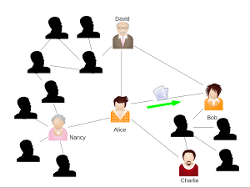
\includegraphics{img/img1.png} 
\caption{A user (Alice) and her contacts (Bob, Charlie, David and Nancy)}
\label{fig:fig1}
\end{figure}

For example consider figure~\ref{fig:fig1} above. In this situation Alice is $P$. Alice has four contacts: Bob, Charlie, David and Nancy, out of which only Bob gets the $update$ $M_P$. Therefore: $C = \{Bob, Charlie, David,Nancy\}$, ${C^+ = \{Bob\}}$ and ${C^- = \{Charlie, David,Nancy\}}$. 

Note that a peer only trusts and has knowledge of its immediate contacts and is not aware of connections between those peers and their contacts. There are practical implementations of the notion of friend-only networks such as Freenet/Darknet \cite{darknet}.

